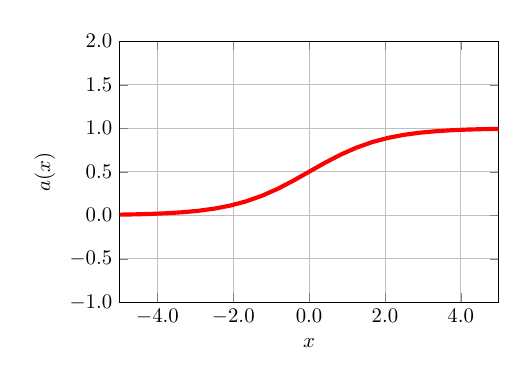
\begin{tikzpicture}[scale=0.75]
\begin{axis}[
width=8cm, height=6cm,
xmin=-5, xmax=5,
ymin=-1.0, ymax=2.0, 
grid, 
xlabel=$x$, ylabel=$a(x)$,
xtick = {-4.0,-2.0,0,2.0,4.0},
ytick = {-1.0,-0.5,...,2.0},
y tick label style={/pgf/number format/.cd,%
        fixed,
        fixed zerofill,
        precision=1},
x tick label style={/pgf/number format/.cd,%
        fixed,
        fixed zerofill,
        precision=1}
]

\addplot[line width=2.pt,color=red]{1/(1+e^(-x))};

% \addplot[red,smooth] gnuplot[id=step]{x>0 ? 1 : -1};

% \addplot[red,smooth] {tanh(x)};

\end{axis}
\end{tikzpicture}